\chapter{Decision trees}\label{appen:DT}
Decision trees are one type of machine learning classifiers \cite{loh2011classification}. They infer the correct class of an observation by a series of yes/no questions, the answer of each question determining the next to ask until a classification is made. These questions, also called rules, are about the values of the observation in a set of variables. We use decision trees in Chapter~\ref{chp:2} to infer whether a species in an ecological network (our observation) will survive or not (the classification) according to their structural properties (the set of variables). Decision trees are convenient for our problem since they do not impose any assumption on the training data, and handle several variables at the same time, even if they are correlated, as some network metrics are \cite{Pichler2022MachineEcologists}.  \\

A trained decision tree starts at a single node called ``root'' node (bottom node in Figure~\ref{app:fig:DT}), which represents a rule for a variable, and then branches in two directions. For example, Rule 1 is ``$k_- > 3$'' in Figure~\ref{chp2:fig:2}. An observation from the data goes to the  right branch of the node if it passes that threshold. Otherwise, it goes to the left. Therefore, each branch corresponds to different possible outcomes, and finishes on new nodes that incorporate more rules on variables until the final classification is achieved at the ``leaves''. \\

The most important variable in predicting the correct class could be deduced from the hierarchy of the nodes. That variable would be the root node, as it can divide the entire data. For example, in Figure~\ref{app:fig:DT}, one could say that the variable involving Rule 1 is the most important as that variable alone can already classify some observations in one class. This rough estimation can only tell us about one variable, and nothing about the following nodes that \textit{just} refine data subsets. However, we can quantify the importance of all the variables if we know some aspects of the training of a decision tree. Explaining this will be a small detour, but it will pay off. \\

\begin{figure}
    \centering
   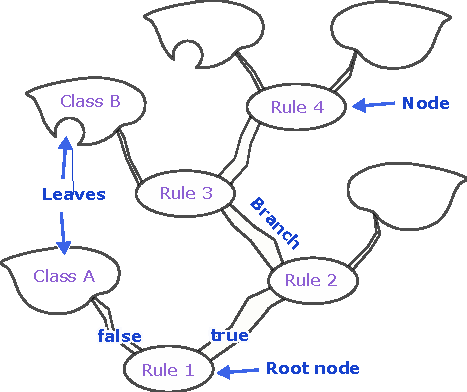
\includegraphics[width=0.8\textwidth]{figures/appendices/DT.pdf}
   
    \caption[Parts of a decision tree]{Parts of a decision tree.}
   \label{app:fig:DT}
\end{figure}

The training of a decision tree is recursive, it follows the same steps for each node. To choose the root node, it scans each variable and tries to divide the training data based on it. Then, the decision tree evaluates each split in light of a ``splitting criterion'' to determine which one performs the best. The splitting criterion we have used is Gini impurity because it favors larger partitions \cite{growingdecisiontrees}. For each branch $b = \{1,2\}$ in a split involving variable $\alpha$, Gini impurity is defined as:

\begin{equation}
   G_b^\alpha = 1- (p_{sur}^2 + p_{ext}^2), 
   \label{eq:ginibalpha}
\end{equation}
where $p_{i}$ is the proportion of observations labeled with class $i = \{sur,ext\}$. We then weigh and sum the Gini impurities of all branches based on the proportion of the data each branch takes up, $d_b$.
\begin{equation}
    G^\alpha  =  d_1 G_1^\alpha + d_2 G_2^\alpha,
    \label{eq:ginialpha}
\end{equation}
where $d_1+d_2=1$. From Eq.\eqref{eq:ginibalpha}, we can see that if a variable can classify all its incoming observations with a single label (a perfect classification), its Gini impurity would be zero and the branch will finish with a leave. For example, the root node in Figure~\ref{chp2:fig:2} (and its schematic version, the Figure~\ref{app:fig:DT}) can directly label some species as ``Surviving''. For all the variables, the one with the smallest impurity will be chosen as the node. Returning to Figure~\ref{chp2:fig:2}, if we constrained the decision tree to just one node, choosing $k_-$ would be the variable that best classifies more species. The logic for all the following nodes is the same. \\

Once the decision tree is constructed, we find in the nodes variables that have a low Gini impurity. Using this concept, the importance $I$ of a variable can be defined as how much each split decreased the impurity. More precisely, it is the difference between the risk for the node (a.k.a. the parent node) and the total risk for its two children nodes \cite{importance}:
\begin{equation}
    I = R_{parent} - R_{child\,1} - R_{child\,2}
    \label{eq:importance}
\end{equation}
In turn, the risk of a node $R_\alpha$ is defined as its impurity weighted by the probability $f_\alpha$ that an observation falls into that node:
\begin{equation}
    R_{\alpha} = G_\alpha f_\alpha
\end{equation}
This probability is just calculated by dividing the number of observations that arrive at the node by the total number of observations in our training data. A node would score one, the maximum importance, if and only if it is the root node (so $f = 1$) and it perfectly splits the data on their labels ($G = 1$ and $R_{child\,1} = R_{child\,2} = 0$). 

Two situations can increase the risk of a node: having high impurity or having a large number of observations passing across it. Nodes at the beginning of a tree will have the highest $f_\alpha$ by definition. The children of these nodes, however, may have still a higher risk than children from nodes near the top that have more chances of a perfect classification. In that way, the importance is less controlled by the order in which nodes appear in the tree. Finally, the most important variable will be the one that minimizes the impurity the most effectively. \\

We can rank the variables according to their importance. But before accepting any ranking, we first need to assess the performance of the decision tree. Ultimately, if the algorithm does not classify the observations with good accuracy, the importance of their variables will the useless. To check the accuracy of the predictions, we create a confusion matrix (Panel a of Fig.\ref{chp2:fig:6}  and \ref{chp2:fig:8}). Its rows correspond to the true class a species belongs to and the columns to the class predicted by the decision tree. Hence, diagonal elements are the percentage of species that are correctly classified, while incorrect predictions are at the off-diagonal elements. \\

To improve the accuracy displayed in the confusion matrix, one could go on growing the tree more and more complex by increasing the number of branches. This would help to better classify the most subtle idiosyncrasies. But when presented with new data, the accuracy of this decision tree would drop. It has been adapted so much to the training data that its predictive power has begun to wane. This is called ``over-fitting'' and it is a crucial aspect of machine learning algorithms' design \cite{spiegelhalter2019art}. In Chapter~\ref{chp:2}, we will train our decision trees for particular types of networks, but we want the results to apply to those types as a whole. \\

There are good practices to avoid over-fitting  \cite{spiegelhalter2019art}. Without giving all the details, we start by randomly dividing our dataset into a training set and a test set. Generally, the training set comprises $80\%$ of the observations The accuracy of the decision tree is now evaluated at the test set, so we can check whether the decision tree is adapting too much to the local circumstances of the training set. A second idea that we have implemented in the construction of the decision tree is ``k-fold cross-validation'' \cite{crossval}. It builds on the idea of testing the algorithm with an independent set. The training dataset is randomly divided into $k$ sets of equal size. Then $k-1$ sets are chosen for training, and this step is repeated $k$ times. The final decision tree is a generalization of the $k$ trees. In this way, the quality of the classification improves since we are systematically removing observations during the construction. \\

Finally, the decision trees have been trained and validated using the \texttt{MATLAB R2021a} algorithms  \texttt{fitctree} \cite{fitctree} and \texttt{crossval} \cite{crossval} from its Statistics and Machine Learning Toolbox.